\documentclass[class=report, crop=false, 12pt,a4paper]{standalone}
\usepackage{enumitem}
\usepackage{float}
\usepackage{graphicx}
\usepackage{multicol}
\usepackage{siunitx}
\usepackage{multirow}
\usepackage{mathtools}
\usepackage{amsmath}
\usepackage{amssymb}
\usepackage{commath}
\usepackage[a4paper,width=150mm,top=25mm,bottom=25mm]{geometry}
\begin{document}
\section{System types}
Specifically, the position error constant $k_p$ and velocity error constant $k_v$ depend upon \textbf{the number of poles at the origin} in the open loop system. These correspond to roots in the denominator at $s=0$, and represent a pure integration. Let's look more generally at the transfer function of our system and introduce the concept of system \textbf{type}. By factoring out any $s$ terms from the denominator, we can write the transfer function in the following form:
\begin{gather}
  G(s)H(s) = \frac{(s-z_1)(s-z_2)(s-z_3)...}{s^p(s-\sigma_1)(s-\sigma_2)(s-\alpha_k + j\omega_k)(s-\alpha_k - j\omega_k)...}
\end{gather}
So, if there are \textit{p poles at the origin}, the system is said to be a 'type p' system.
\begin{quote}
  System type IS NOT THE ORDER OF THE SYSTEM!
\end{quote}
For example, the servo motor can be expressed as:
\begin{gather}
  \frac{\Theta_0(s)}{\Theta_i(s)}=\frac{k}{s(Is +f)}
\end{gather}
which is a type 1 system. The electromagnet from lecture 2 can be expressed as:
\begin{gather}
  \frac{I(s)}{V(s)} = \frac{1}{Ls +R}
\end{gather}
which is a type 0 system. The mas spring damper system can be expressed as:
\begin{gather}
  \frac{X(s)}{F(s)} = \frac{1}{ms^2 + cs + k}
\end{gather}
which is a type 0 system.

The system type quickly tells us the form of the SSE for our inputs without manipulation of block diagrams or converting to time domain. This gives an indication of the design of the controller. 
\subsection{System type - calculating error}
Essentially, for a zero error we want $k_p$ and $k_v$ to be infinite, or at least be a constant for a finite error, depending on our requirements. 
\begin{gather}
  SSE = \frac{a}{1+ k_p}, \ SSVL = \frac{a}{k_v}\\
  k_p = \lim_{s\rightarrow 0} G(s)H(s), \ k_v = \lim_{s\rightarrow 0}sG(s)H(s)
\end{gather}
\subsection{System type for unit feedback control systems - calculating error}
The \textbf{position error constant} $k_p$ for a \textit{type p system} is given by: 
\begin{itemize}
  \item $p > 0, \ k_p = \lim_{s\rightarrow 0} G(s) = \infty$ - no steady-state position error
  \item $p=0, \ k_p$ is finite - finite position error
\end{itemize}
The \textbf{velocity error constant} for a \textit{type p} system is given by:
\begin{itemize}
  \item $p> 1, \ k_v = \lim_{s\rightarrow 0} sG(s) = \infty$ - no velocity error
  \item $p = 1, \ k_v$ is finite - steady state velocity lag
  \item $p = 0, \ k_v = 0$ infinite lag (completely fails to track) 
\end{itemize}
\begin{table}[H]
  \begin{center}
  \begin{tabular}{|c|c|c|c|}
    \hline
    & \multicolumn{3}{c|}{Input type}\\
    \cline{2-4}
    No. Integrators & Step & Ramp & Acceleration\\
    in denominator & $r(t) = a$ & $r(t) = at$ & $r(t) = \frac{at^2}{2}$\\
    = system TYPE & $R(s) = \frac{a}{s}$ & $R(s) = \frac{a}{s^2}$ & $R(s) = \frac{a}{s^3}$\\
    \hline
    \hline
    0 & $e_{ss} = \frac{a}{1+k_p}$ & $e_{ss} = \infty$ & $e_{ss} = \infty$\\
    \hline
    1 & $e_{ss} = 0$ & $e_{ss} = \frac{a}{k_v}$ & $e_{ss} = \infty$\\
    \hline
    2 & $e_{ss} = 0$ & $e_{ss} = 0$ & $e_{ss} = \frac{a}{k_a}$\\
    \hline
  \end{tabular}
  \end{center}
  \caption{}
\end{table}
where $\infty$ means the system never settles. The more poles there are at the origin of the open-loop system, the better steady-state tracking performance. However, pure integrations have a highly destabilising effect on the control system!
\subsection{Type 0 servo - spring return}
Previously we have looked at servos with inertia and damping only, without and compliance/springs. This gives a type-1 transfer function. However, when a spring is added, the system becomes type-0.
\begin{equation}
  \frac{\Theta_0(s)}{\Theta_i(s)} = \frac{k}{s(Is + f)}
\end{equation}
The question arises, why would you add a spring? Some systems are not bidirectional e.g. a single acting piston in a hydraulic system. A spring is needed to return the piston to the correct position in the cycle. A spring is often added to servo actuators to return to a given position when system is off. HVAC systems use this for fire safety. The transfer function of this servo now becomes:
\begin{gather}
  \sum T = I \frac{\textrm{d}^2 \theta_0}{\textrm{d} t^2}\\
  I \frac{\textrm{d}^2 \theta_0}{\textrm{d}t^2} = T_s + T_f + T_m
\end{gather}
where $T_s$ and $T_f$ oppose the motion of the motor. In time domain:
\begin{equation}
  I \frac{\textrm{d}^2 \theta_0}{\textrm{d}t^2} = - k_s \theta_0 - f \frac{\textrm{d}\theta_0}{\textrm{d} t} + k_m \theta_i
\end{equation}
In Laplace:
\begin{gather}
  Is^2\Theta_0(s) = -k\Theta_0(s) - fs\Theta_0(s)+ k_m\Theta_i(s)\\
  Is^2 \Theta_0(s) + k_s \Theta_0(s) + fs\Theta_0(s) = k_m \Theta_i(s)\\
  \Theta_0(s) \left(Is^2 + k_s + fs\right) = k_m \Theta_i(s)
\end{gather}
Transfer function:
\begin{equation}
  \frac{\Theta_0(s)}{\Theta_i(s)} = \frac{k_m}{Is^2 + fs + k_s} = G(s)
\end{equation}
So the closed loop transfer function is now:
\begin{figure}[H]
  \centerline{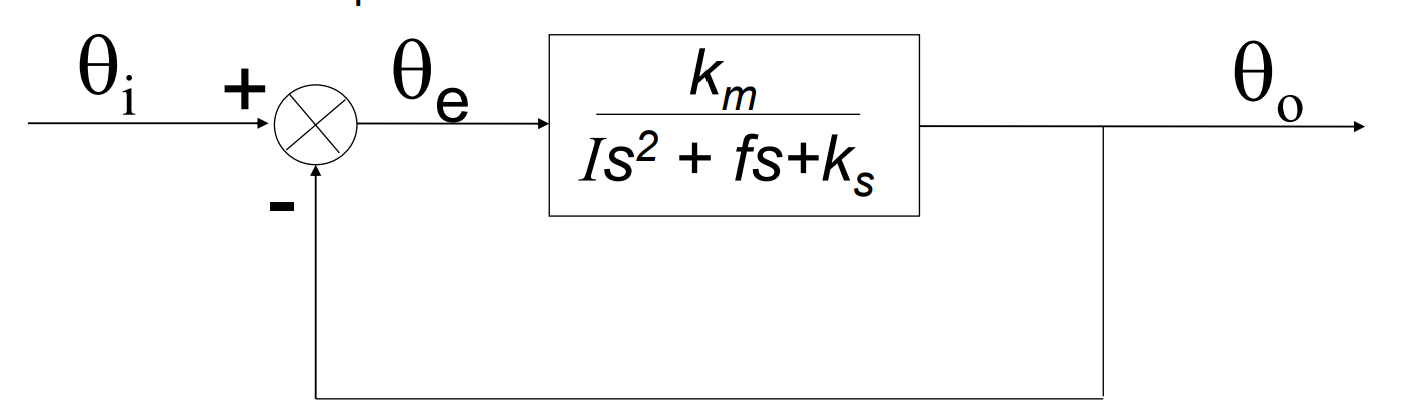
\includegraphics[width = 0.8\textwidth]{../img/diagram108.png}}
  \caption{}
\end{figure}
\begin{gather}
  F(s) = \frac{G(s)}{1 + G(s)} = \frac{k_m}{Is^2 + fs + k_s + k_m}\\
  k_p = \lim_{s\rightarrow 0}G(s)H(s) = \frac{k_m}{Is^2 + fs+ k_s} = \frac{k_m}{k_s}\\
  k_v = \lim_{s\rightarrow 0} sG(s) H(s) = \frac{sk_m}{Is^2 + fs + k_s} = \frac{0}{k_s}\\
  SSE = \frac{a}{1 + k_p} = \frac{ak_s}{k_s + k_m}, \ SSVL = \frac{a}{k_v} = \infty
\end{gather}
So now the servo will now only travel a fraction of the required distance for a step input, and will completely fail to track a ramp input, never settling to a steady state. We need an improved controller for these systems!
\section{Proportional control}
\subsection{Proportional control - damping ratio trade off}
We have seen the effect of damping ratio for our simple servo control system so far. We have two conflicting requirements:
\begin{itemize}
  \item For transient response we want something around 0.6-0.8 to reduce overshoot and oscillations. $\zeta = \frac{f}{2\sqrt{kI}}$
  \item For steady state response, we want the damping ratio as low as possible at the expense of oscillations. $SSVL = \frac{af}{k} = \frac{2\zeta a }{\omega_n}$
\end{itemize}
For our type 1 servo, this trade off occurs if we want good ramp tracking, something we could possibly neglect in certain applications. However, the type 0 servo SSVL  renders it close to unusable in most control applications (with the current controller). Commonly the challenge is to increase $\zeta$, but with our current system, we do not have many options for adjustment. 
\begin{figure}[H]
  \centerline{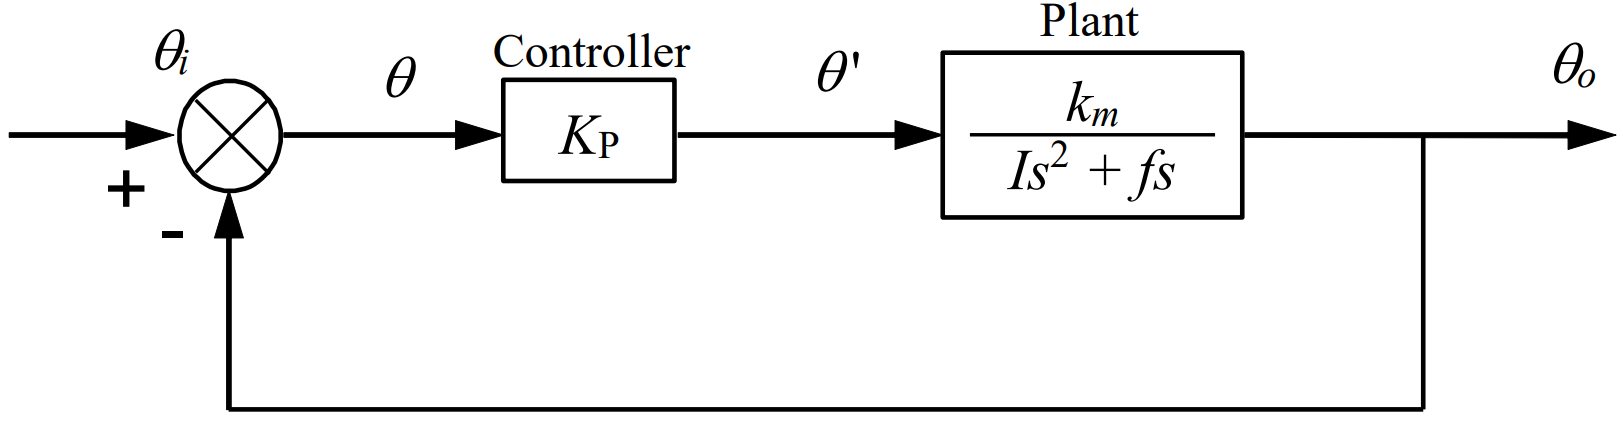
\includegraphics[width = 0.8\textwidth]{../img/diagram109.png}}
  \caption{}
\end{figure}
We can either increase our friction $f$ but this increases wear on the components, reducing the life of the system. So that leaves the controller gain $k_p$ to adjust, we can reduce it at the expense of steady state performance. So we need a better controller!
\section{Velocity feedback}
\subsection{Doing better - compensation methods}
What the controller we have seen so far is known as a proportional controller, the control signal is directly proportional to the error signal, scaled by $k_p$. Compensation methods have been designed to improve \textbf{both} transient and steady state performance. One of the earliest and simplest compensation methods is to consider not just the position but the velocity too. 
\begin{figure}[H]
  \centerline{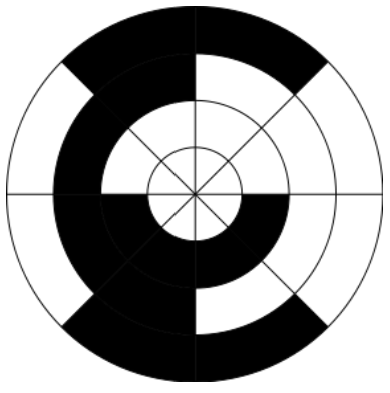
\includegraphics[width = 0.2\textwidth]{../img/diagram110.png}}
  \caption{}
\end{figure}
If we take the position from the shaft encoder, and also record the change over time, we can measure the speed. The block diagram of this is just $s$ - as this is the differential operator, we also include another gain here $k_{vel}$ so we can choose the relative contributions of the two feedbacks. So we have the following block diagram.
\begin{figure}[H]
  \centerline{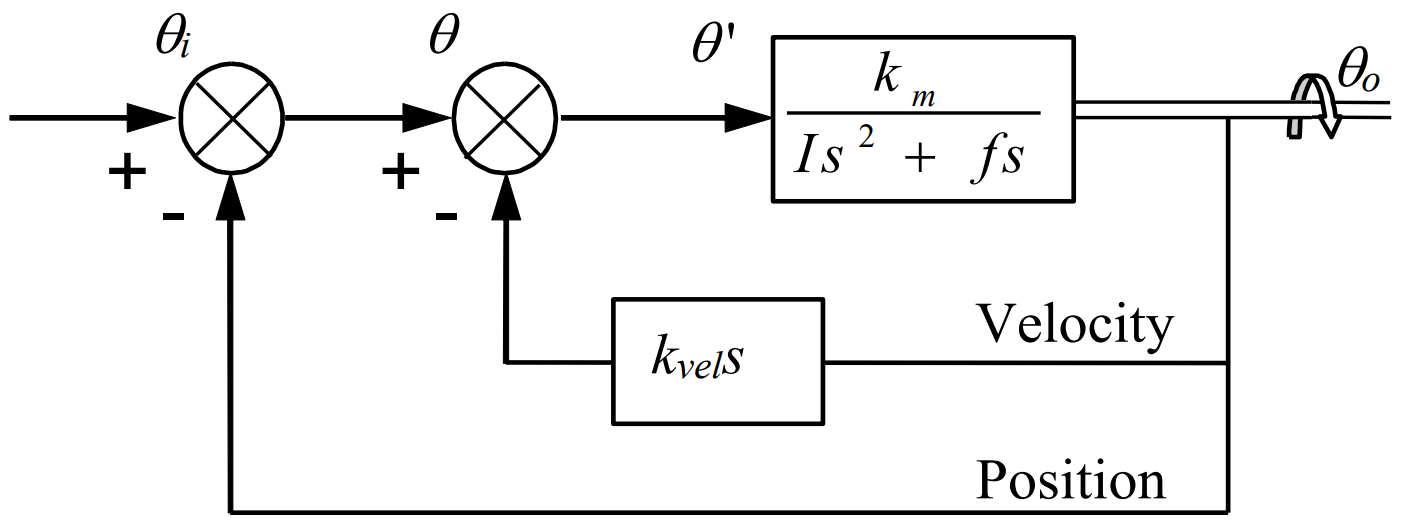
\includegraphics[width = 0.8\textwidth]{../img/diagram111.png}}
  \caption{}
\end{figure}
Inner comparator:
\begin{equation}
  \theta ' = \theta - k_{vel} s \theta_0
\end{equation}
Outer comparator:
\begin{equation}
  \theta = \theta_i - \theta_0
\end{equation}
If we calculate the new closed loop transfer function - work outwards!
\begin{align}
  \frac{\theta_0}{\theta} &= \frac{G}{1 +GH} = F(s)\\
  F(s) &= \frac{\frac{k_m}{Is^2 + fs}}{1 + \frac{k_m}{Is^2 + fs}k_{vel} s} = \frac{k_m}{Is^2 + fs + k_m k_{vel}s}\\
  &= \frac{k_m}{Is^2 + \left(f + k_m k_{vel}\right) s}
\end{align}
\begin{figure}[H]
  \centerline{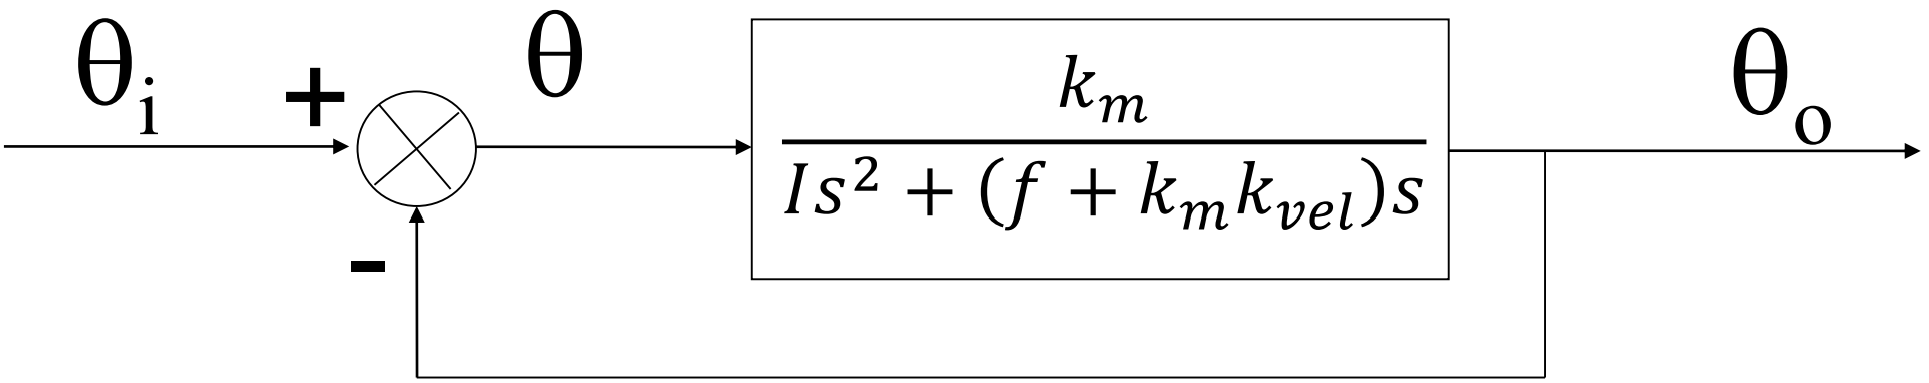
\includegraphics[width = 0.8\textwidth]{../img/diagram112.png}}
  \caption{}
\end{figure}
Inner loop transfer function:
\begin{equation}
  F(s) = \frac{k_m}{Is^2 + \left(f + k_m k_{vel}\right) s}
\end{equation}
Total closed loop transfer function:
\begin{gather}
  F_T(s) = \frac{F}{1 + F}\\
  F_T(s) = \frac{k_m}{Is^2 + (f+k_m k_{vel})s + k_m}\\
  F_T(s) = \frac{\frac{k_m}{I}}{s^2 + \frac{\left(f + k_m k_{vel}\right)}{I} s + \frac{k_m}{I}}\\
  \omega_n = \sqrt{\frac{k_m}{I}}, \ \zeta = \frac{f + k_m k_{vel}}{2 \sqrt{kI}}
\end{gather}
So by adding the extra loop, we are able to keep the natural frequency the same, \textit{but increase the damping ratio}. This means we can greatly improve the transient response compared to proportional control, where we can only scale the motor gain $k_m$ through adjusting the parameter $k_p$. This is evident when considering the position of the poles of the system on the s-plane. Adjusting the motor gain using proportional control $\left( k_p\right)$ can only move the poles closer to the real axis. But using velocity feedback $\left( k_{vel}\right)$, it is possible to move the poles away from the imaginary axis, thus reducing the decay time. 
\begin{figure}[H]
  \centerline{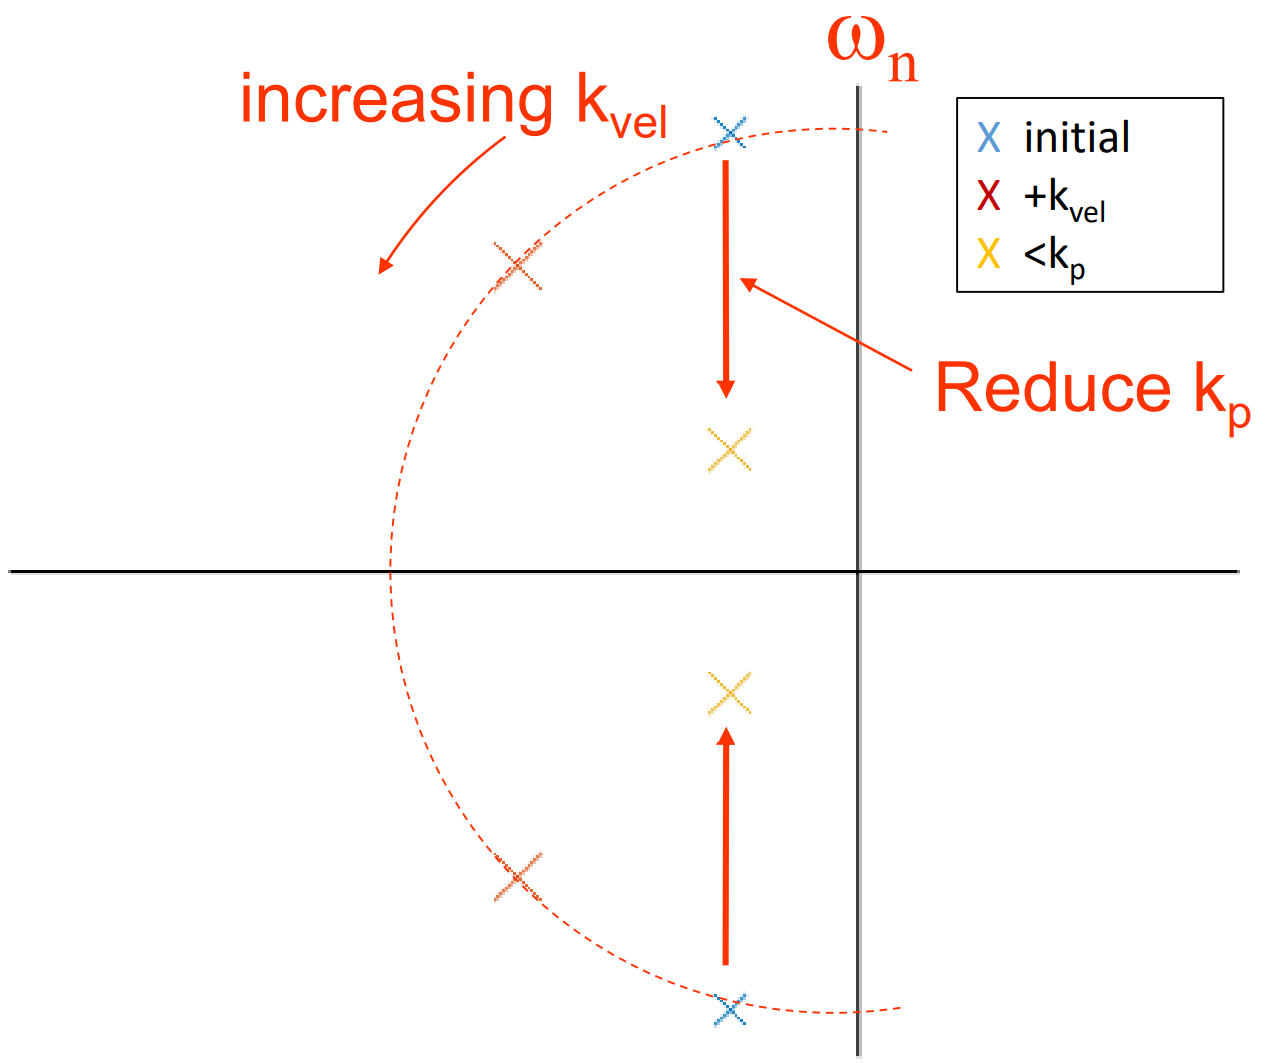
\includegraphics[width = 0.5\textwidth]{../img/diagram113.png}}
  \caption{}
\end{figure}
In this example, the initial zeta was $\zeta = 0.3$, in order to achieve the practical estimate of $\zeta = 0.7$ with proportional control, we have to increase both the rise time and settling time. However, with velocity feedback we can achieve a vastly improved transient response.
\begin{figure}[H]
  \centerline{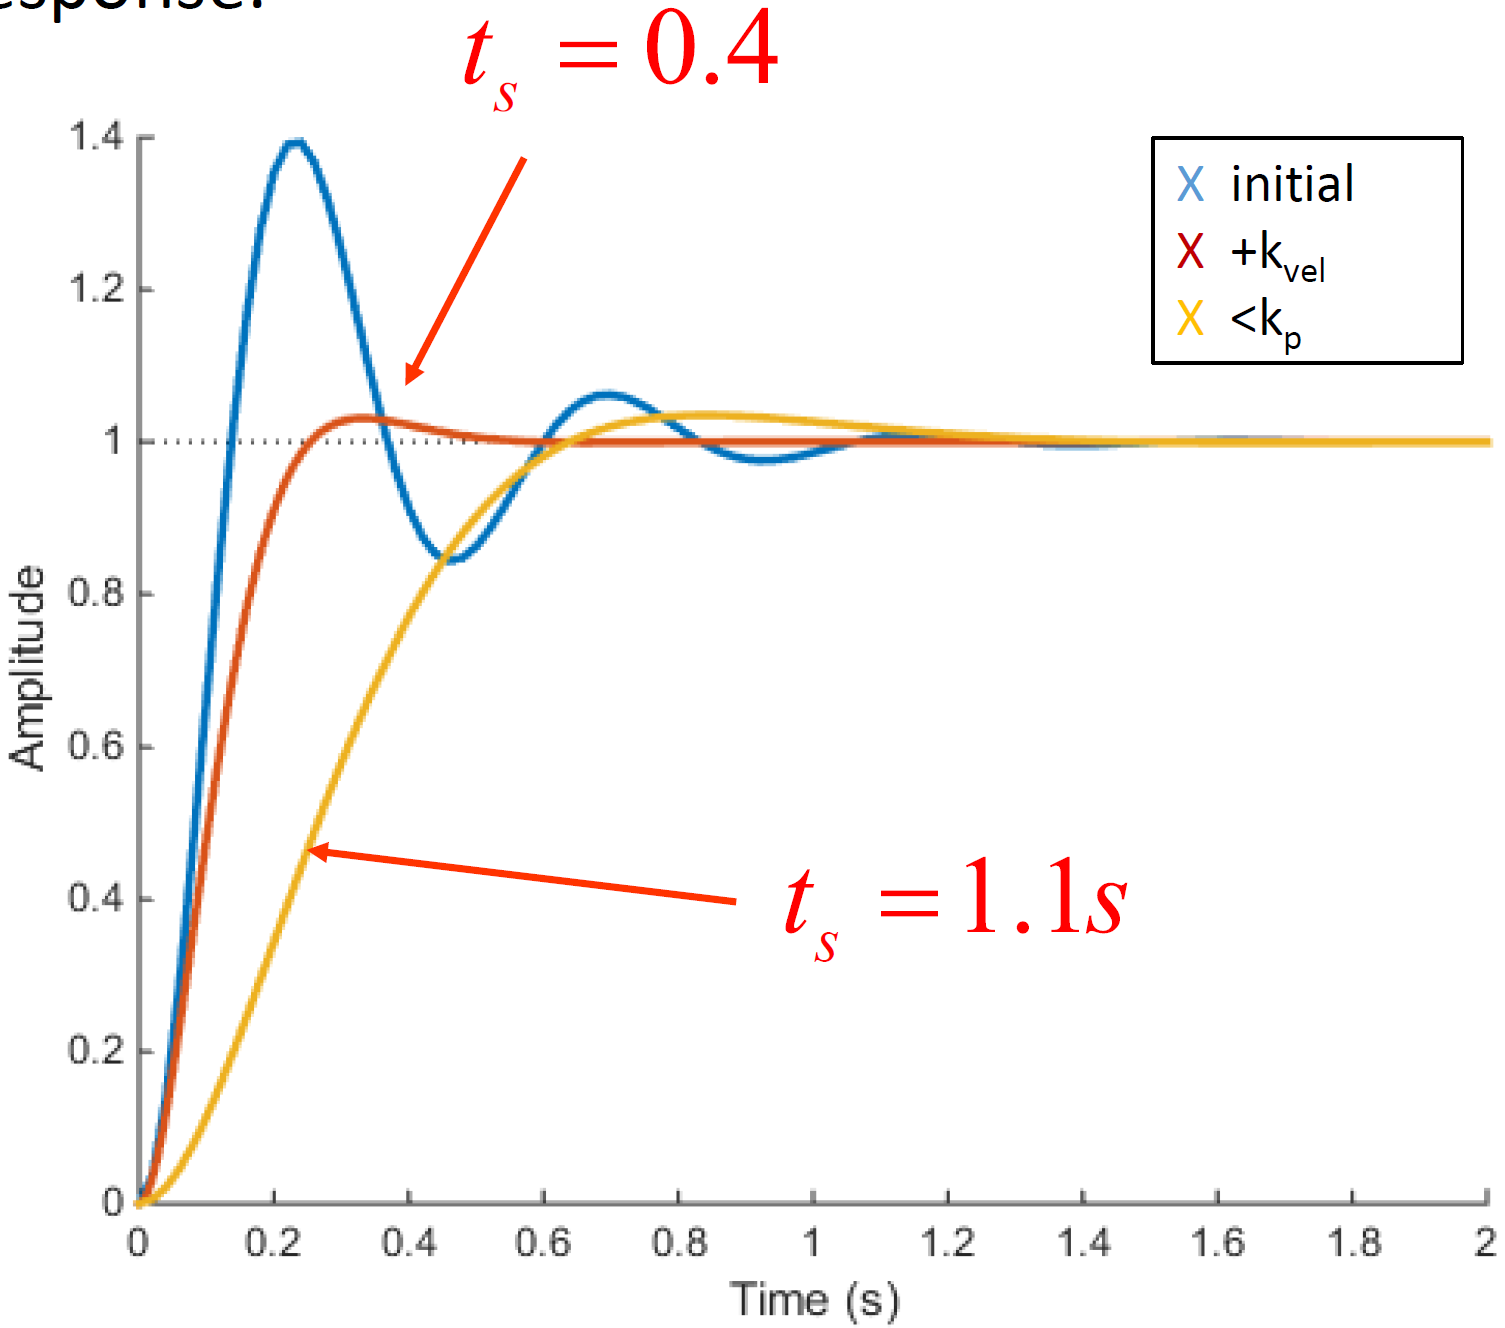
\includegraphics[width = 0.5\textwidth]{../img/diagram114.png}}
  \caption{}
\end{figure}
\subsection{Velocity feedback - disadvantages}
This improved transient response comes at the expense of the steady state error, the expression for the SSVL becomes:
\begin{gather}
  k_v = \lim_{s\rightarrow 0} s F(s) = \frac{sk_m}{Is^2 + \left( f + k_m k_{vel}\right)s} = \frac{k_m}{f + k_m k_{vel}}\\
  SSVL = a \frac{k_m}{f + k_m k_{vel}}
\end{gather}
Compare this SSVL to the one we had previously $\left( \frac{af}{k}\right)$. Using this feedback system allows for the designer to trade off the transient and steady state response dependent upon the requirements of the system. However, using the velocity in this manner is very sensitive to errors or noise from the sensor, which give large instantaneous changes in the error signal. To combat this, a low pass filter is normally employed in the feedback loop before the derivative term. 
\begin{figure}[H]
  \centerline{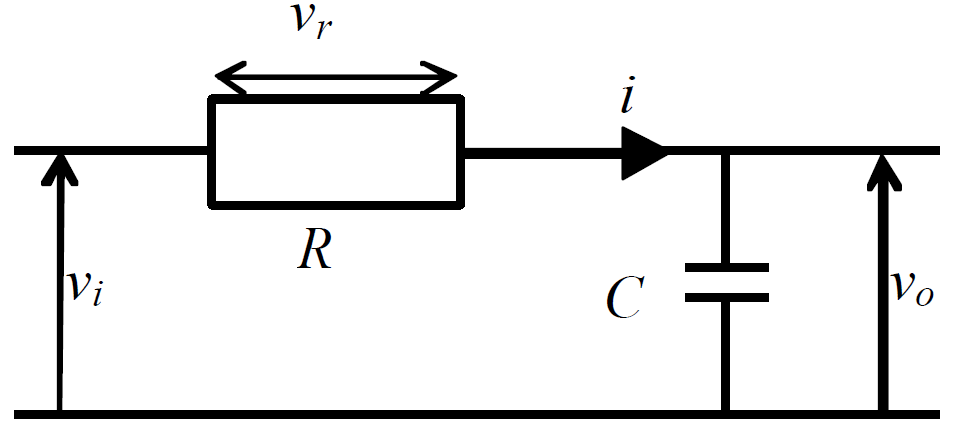
\includegraphics[width = 0.4\textwidth]{../img/diagram115.png}}
  \caption{}
\end{figure}
\begin{gather}
  = \frac{1}{RCs + 1} \textrm{ see lecture 2}
\end{gather}
This makes the response more complex and slightly reduces the improvements in transient response obtained.
\subsection{Alternative controllers}
The velocity feedback is rather specific to servomechanisms with a shaft encoder. It is not always possible to have a sensor or a measurement from which both the variable and the derivative can be acquired simultaneously. 
\begin{figure}[H]
  \centerline{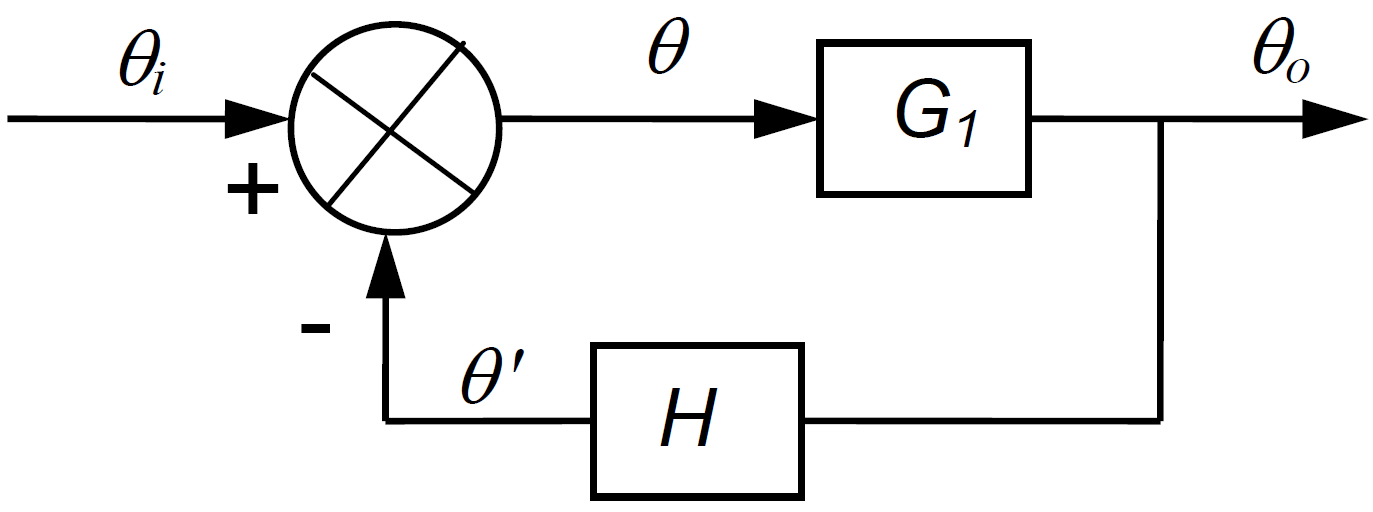
\includegraphics[width = 0.6\textwidth]{../img/diagram116.png}}
  \caption{}
\end{figure}
Instead, we can consider what happens to the \textit{error} across time - something necessarily present in all closed loop systems!
\section{PID control}
PID = Proportional, Integral and Derivative controllers: These controllers consist of three terms, all applied to the error signal. They are \textit{incredibly} common in engineering, accounting for nearly 90\% of all use cases. 
\subsection{Working example: PID control for servo-mechanism}
These can be modelled as shown below, with a DC motor rotating an inertial load, with a friction or damping resistance.
\begin{figure}[H]
  \centerline{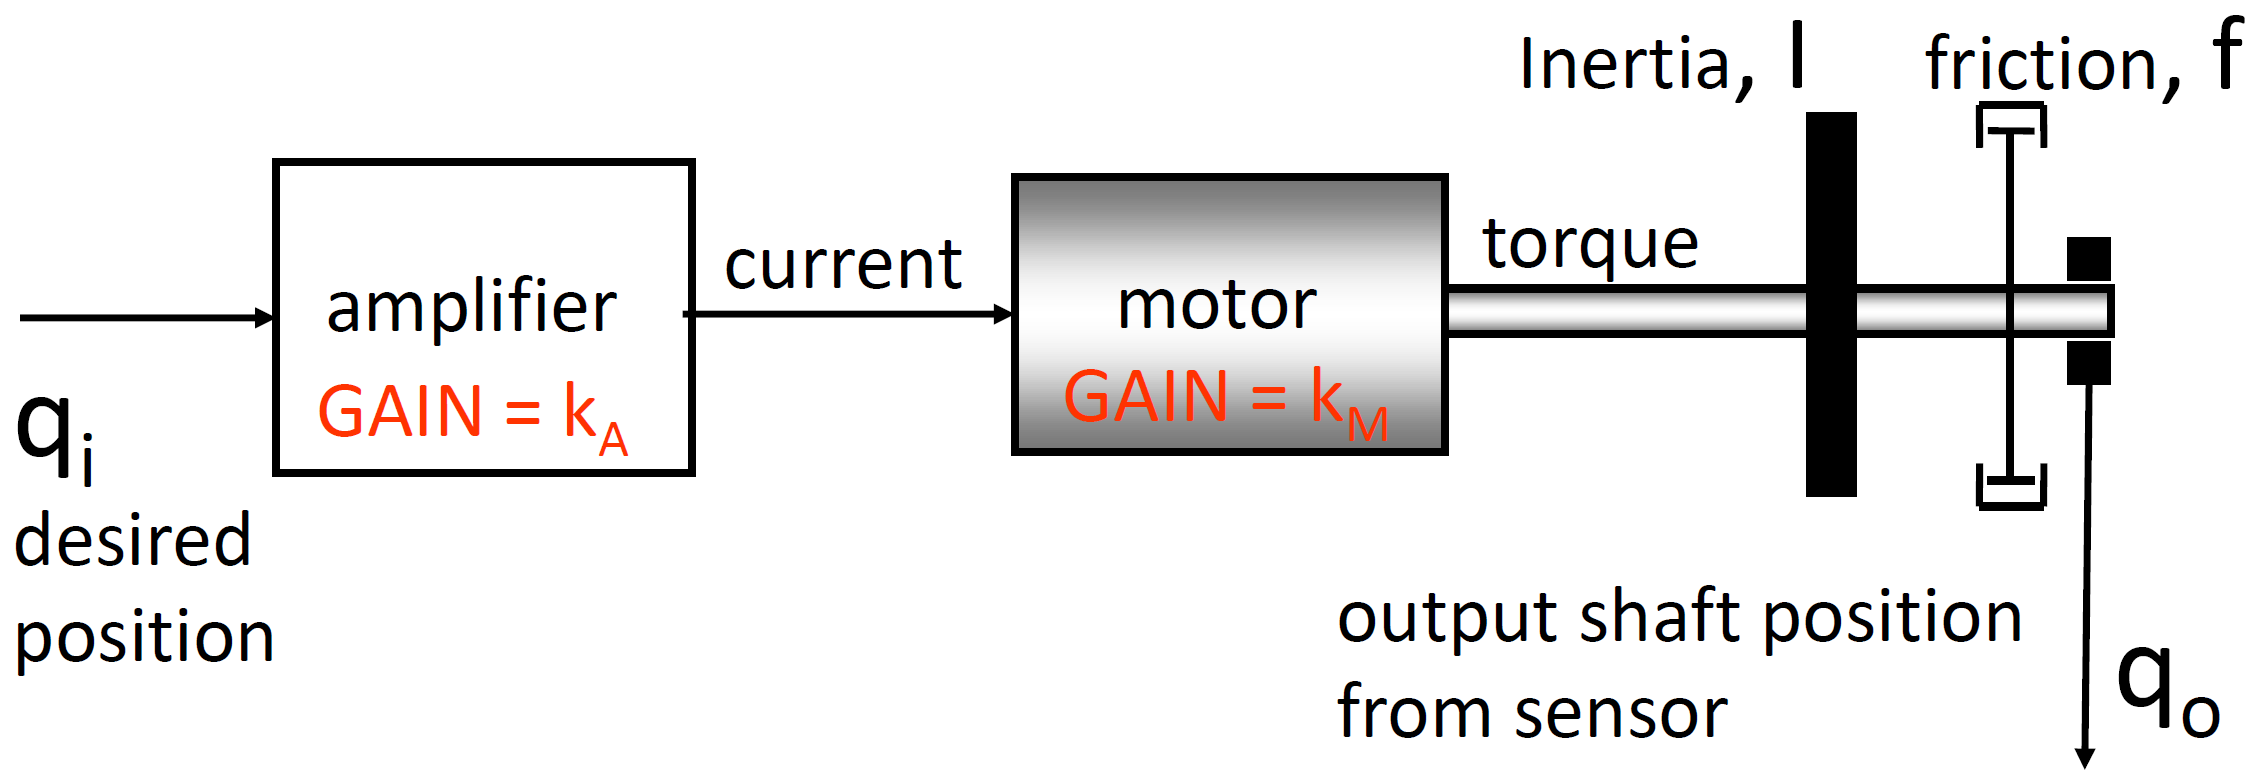
\includegraphics[width = 0.8\textwidth]{../img/diagram117.png}}
  \caption{}
\end{figure}
\subsection{Proportional error}
\begin{figure}[H]
  \centerline{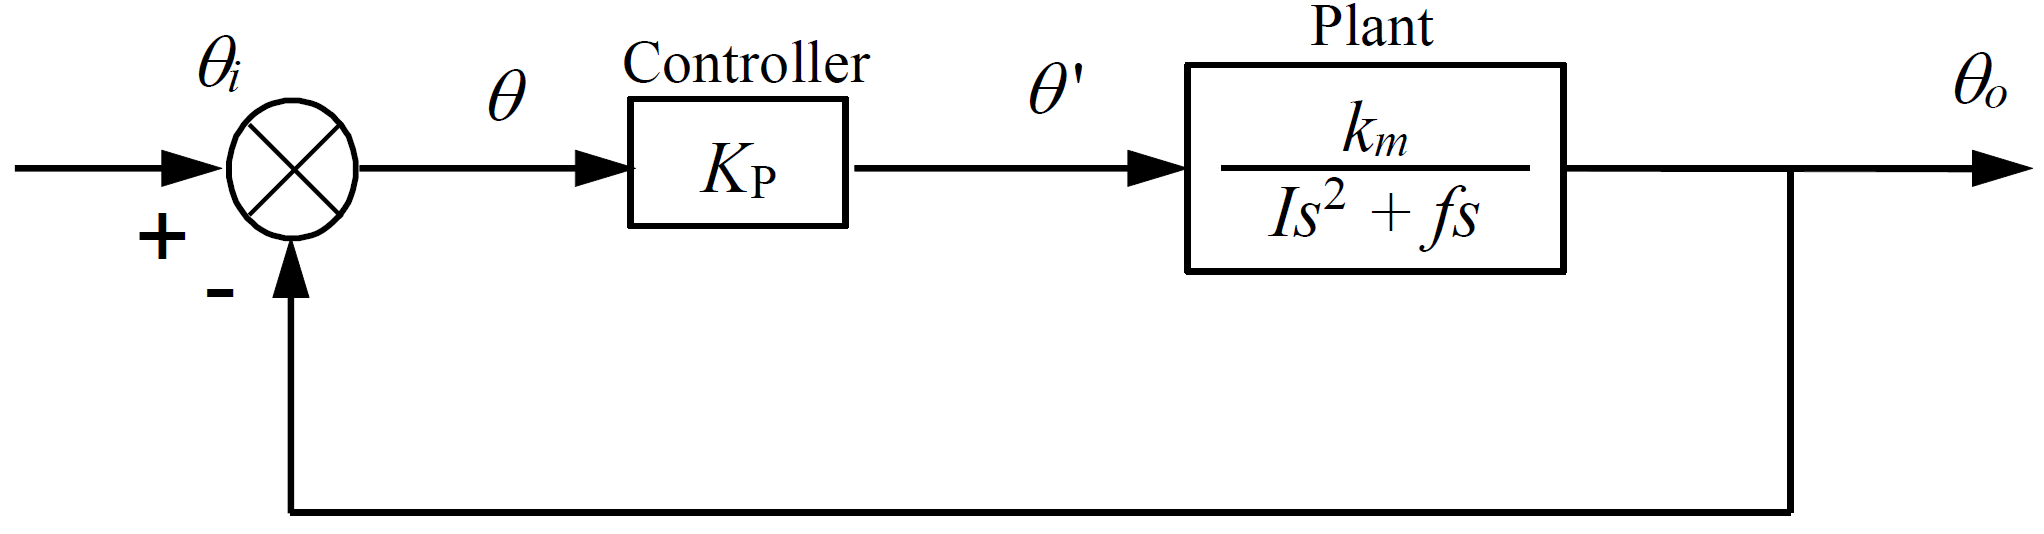
\includegraphics[width = 0.8\textwidth]{../img/diagram118.png}}
  \caption{}
\end{figure}
\begin{gather}
  F(s) = \frac{G(s)}{1+ G(S)} = \frac{k_p k_m}{Is^2 + fs + k_p k_m}
\end{gather}
We have already seen this in our previous analysis of second order systems, and from changing $k_m$ from last last week. To summarise: low values of $k_p$ give stable but slow responses, and high SSVL. High values reduce SSVL but response overshoots considerably. With proportional control the error \textit{and thus the control signal} does not reach zero until the motor is at the desired position.
\begin{figure}[H]
  \centerline{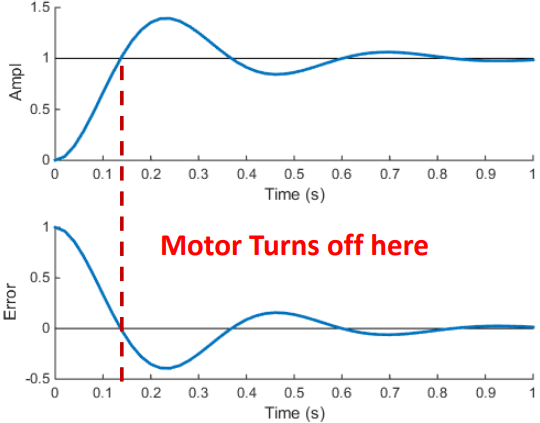
\includegraphics[width = 0.6\textwidth]{../img/diagram119.png}}
  \caption{}
\end{figure}
However, due to the inertia for the system, the motor continues to move even without a control signal, resulting in an overshoot.
\subsection{PID control}
\begin{figure}[H]
  \centerline{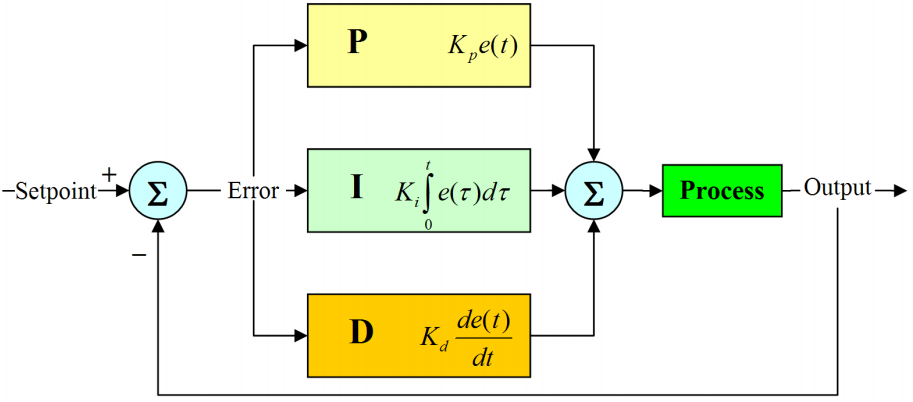
\includegraphics[width = 0.8\textwidth]{../img/diagram120.png}}
  \caption{}
\end{figure}
\subsection{Derivative error}
We can replicate this by considering the \textbf{derivative} of the error. 
\begin{figure}[H]
  \centerline{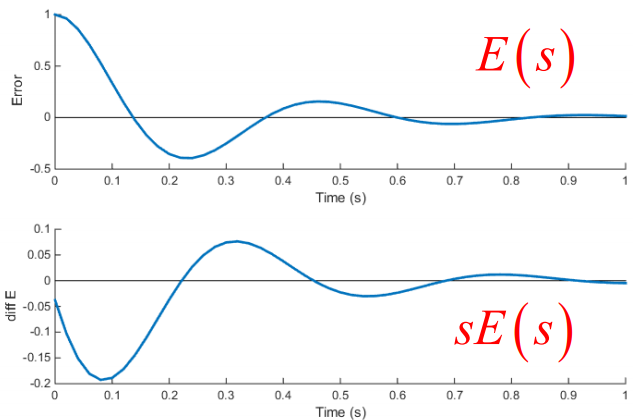
\includegraphics[width = 0.8\textwidth]{../img/diagram121.png}}
  \caption{}
\end{figure}
This is negative as the servo approaches the target, so offers a way of restraining the servos forward motion. Lets consider a derivative controller with unity proportional gain.
\begin{figure}[H]
  \centerline{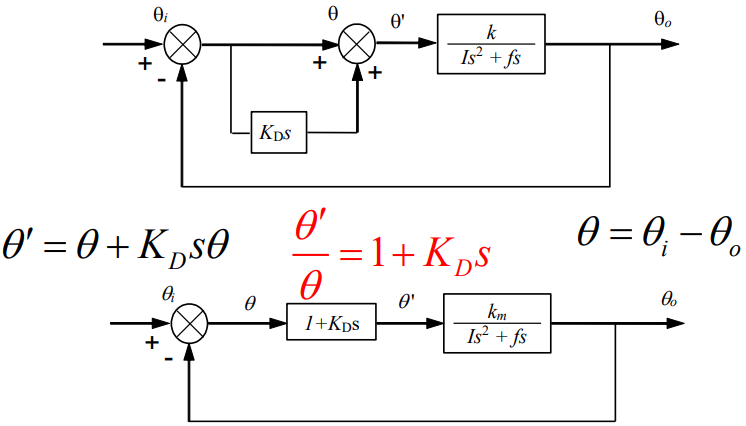
\includegraphics[width = 0.8\textwidth]{../img/diagram122.png}}
  \caption{}
\end{figure}
The open loop transfer function now becomes type 1: 
\begin{equation}
  G' = \frac{\left( 1 + K_D s \right) k_m}{Is^2 + fs}
\end{equation}
Giving a \textit{closed loop transfer function} of:
\begin{gather}
  F(s) = \frac{G'(s)}{1 + G'(s)} = \frac{\left( 1 + K_D s \right)k_m}{Is^2 + fs + \left( 1+K_D s\right)k_m}\\
  F(s) = \frac{k_m K_d s + k_m}{Is^2 + \left( f + k_m K_D\right)s + k_m}
\end{gather}
System is still second order but now there is a zero in the numerator. The effect of this is subtle compared to the change in the poles. More importantly, lets consider the SSVL of this system:
\begin{align}
  k_v = \lim_{s\rightarrow 0} s G'(s) = \frac{s \left( 1+K_D s\right) k_m}{s\left( Is + f \right)} = \frac{k_m}{f}
\end{align}
So, unlike velocity feedback, the SSVL is unchanged by derivative error. So we can improve transient response without compromising steady state error. The effect on the step response is similar to that of the minor loop velocity feedback.
\begin{figure}[H]
  \centerline{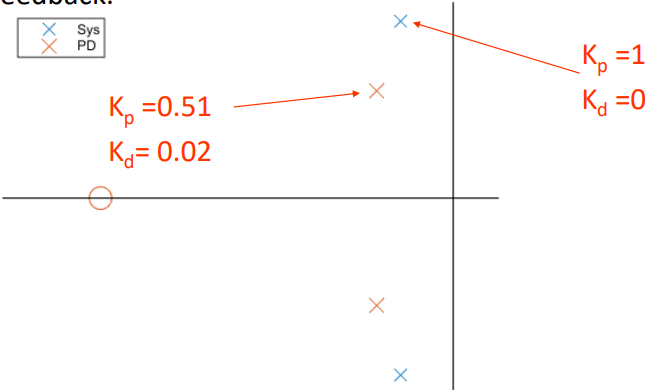
\includegraphics[width = 0.6\textwidth]{../img/diagram123.png}}
  \caption{}
\end{figure}
The poles of the system become less oscillatory and decay quicker. This combined with a reduced proportional gain, gives an improved transient response. This is clear when looking at the step response, and the relative contributions of the two error terms.
\begin{figure}[H]
  \centerline{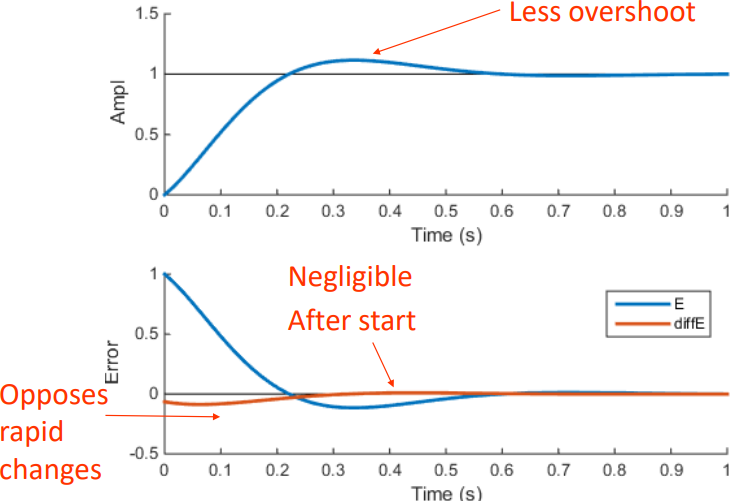
\includegraphics[width = 0.6\textwidth]{../img/diagram124.png}}
  \caption{}
\end{figure}
At the start, the derivative term is significant \textit{and in the opposite direction to} the proportional error term, but becomes negligible as the system settles.
\subsection{PID control}
\begin{figure}[H]
  \centerline{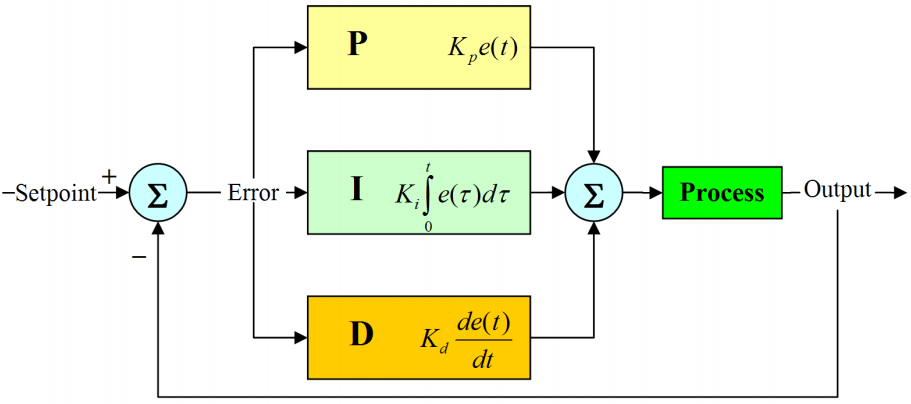
\includegraphics[width = 0.6\textwidth]{../img/diagram125.png}}
  \caption{}
\end{figure}
\subsection{Integral error}
\begin{figure}[H]
  \centerline{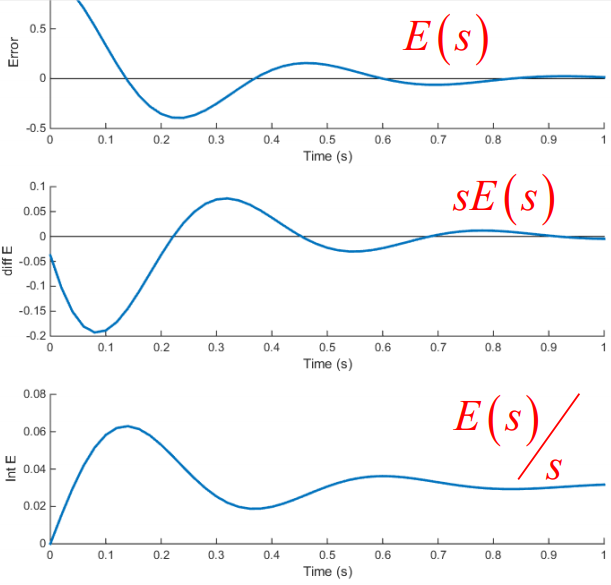
\includegraphics[width = 0.6\textwidth]{../img/diagram126.png}}
  \caption{}
\end{figure}
Further, if we consider the \textbf{integral} or total error over time. This gradually increases over time, and can be used to magnify the control signal for small errors, and improve SSE. The integral of the error is used for correcting steady state errors, as it adds a pole at zero in the transfer function. This increases type.
\begin{figure}[H]
  \centerline{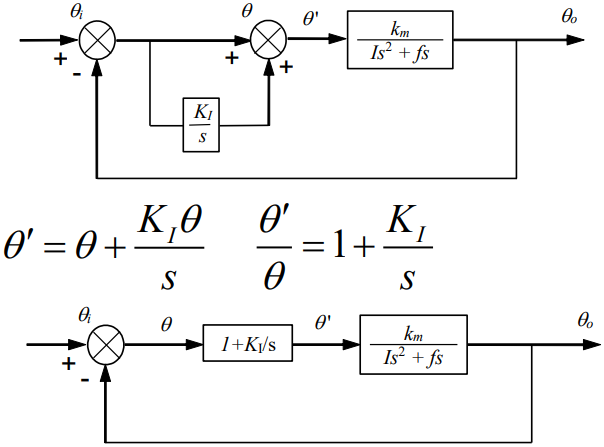
\includegraphics[width = 0.6\textwidth]{../img/diagram127.png}}
  \caption{}
\end{figure}
\begin{gather}
  G' = \frac{\left(1 + \frac{K_I}{s}\right) k_m}{Is^2 + fs} = \frac{\frac{1}{s} \left(s + K_I \right)k_m}{s \left(Is + f\right)}\\
  G' = \frac{k_m s + k_m K_I}{s^2 \left(Is + f\right)}
\end{gather}
With a closed loop transfer function of:
\begin{gather}
  F(s) = \frac{G'(s)}{1 + G'(s)} = \frac{k_m s + k_m K_I}{s^2 \left( Is + f\right) + k_m s +k_m K_I}\\
  F(s) = \frac{K-m s + k_m K_I}{Is^3 + fs^2 + k_m s + k_m K_I} \label{3rdOTF}
\end{gather}
Eq.\ref{3rdOTF} is a third order transfer function. Increasing the system type improves the steady state response:
\begin{gather}
  k_v = \lim_{s\rightarrow 0} sG'(s) = \frac{s\left( k_m s + k_m K_I \right)}{s^2 \left( Is + f \right)}\\
  k_v = \frac{k_m K_I}{0} = \infty \\
  \textrm{SSVL} = \frac{a}{k_v} = 0
\end{gather}
We now have no velocity lag! The effect of an extra pole close to the origin - which would make our system \textit{very slow} - is largely cancelled out by the nearby zero. 
\begin{figure}[H]
  \centerline{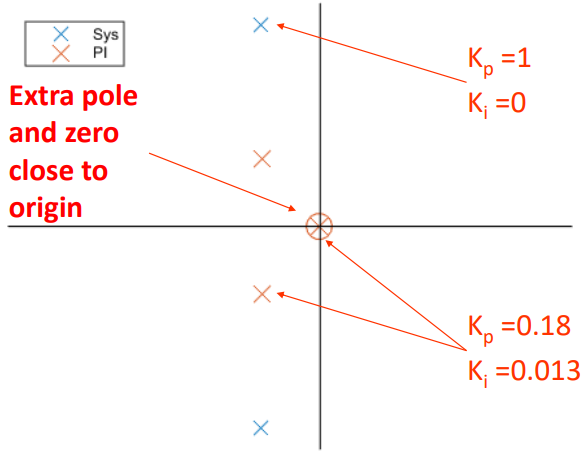
\includegraphics[width = 0.6\textwidth]{../img/diagram128.png}}
  \caption{}
\end{figure}
This means the system is broadly similar to a proportional controller, with the exception of improved steady state performance.
\begin{figure}[H]
  \centerline{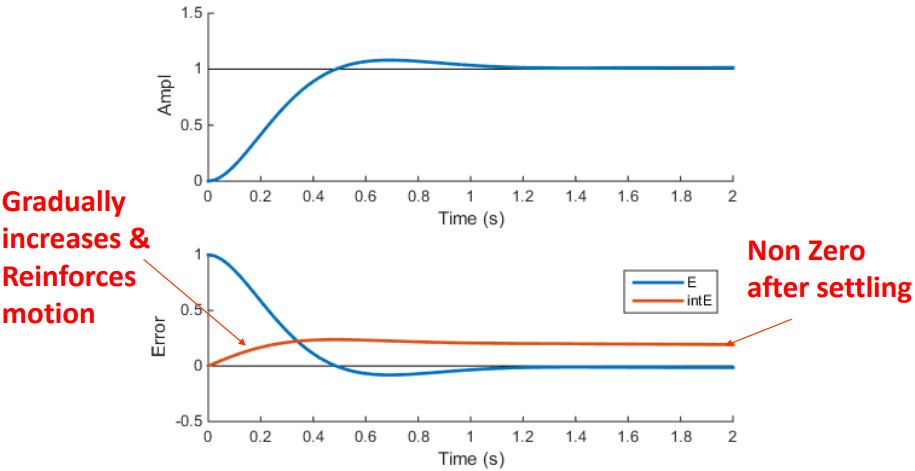
\includegraphics[width = 0.6\textwidth]{../img/diagram129.png}}
  \caption{}
\end{figure}
We can see that the integral term has enabled proper tracking of a ramp input.
\begin{figure}[H]
  \centerline{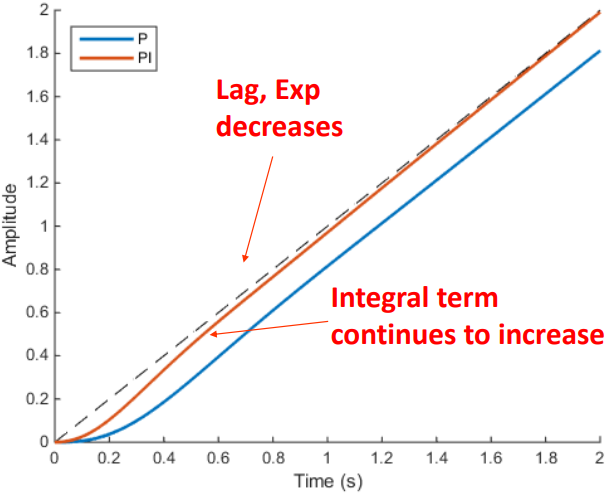
\includegraphics[width = 0.6\textwidth]{../img/diagram130.png}}
  \caption{}
\end{figure}
This is useful for overcoming steady state errors arising from nonlinearities not included in the model which prevent proper tracking in reality.
\subsection{PID control}
Putting all three of these controllers together gives the complete PID.
\begin{figure}[H]
  \centerline{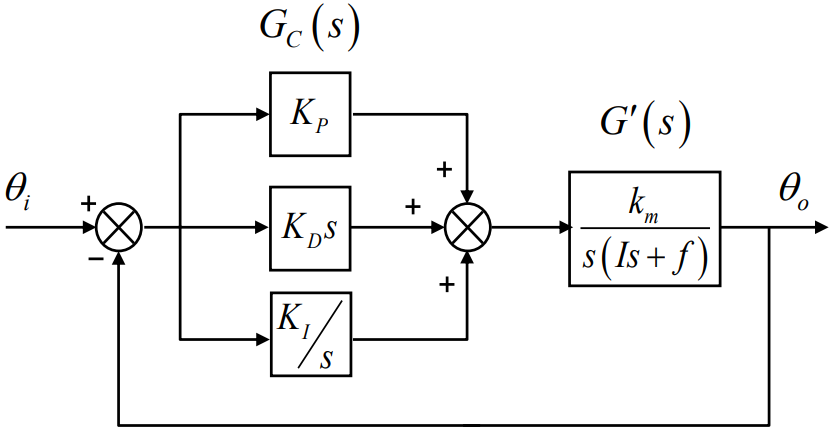
\includegraphics[width = 0.6\textwidth]{../img/diagram131.png}}
  \caption{}
\end{figure}
\begin{align}
  G_c (s) = K_P + K_D s + \frac{K_I}{s} = \frac{K_D s^2 + K_P s + K_I}{s}
\end{align}
Open loop gain:
\begin{align}
  G'(s) = \frac{k_m \left( K_D s^2 + K_P s + K_I \right)}{s^2 \left( Is + f \right)}
\end{align}
The closed loop transfer function is then:
\begin{align}
  F(s) &= \frac{k_m \left(K_D s^2 + K_P s + K_I\right)}{s^2 \left( Is + f\right) + k_m \left(K_D s^2 + K_P s +K_I \right)}\\
  F(s) &= \frac{k_m K_D s^2 + k_m K_P s + k_m K_I}{Is^3 + fs^2 + k_m K_D s^2 + k_m K_P s + k_m K_I}\\
  F(s) &= \frac{k_m K_D s^2 + k_m K_P s + k_m K_I}{Is^3 + \left( f +k_m K_D\right) s^2 + k_m K_P s + k_m K_I}
\end{align}
Thus, by choosing the appropriate values of $K_P$, $K_D$ and $K_I$, it is possible to design a controller with improved transient response \textbf{and} decreased/no steady state error (in theory). There is no unique solution for the settings of the three gains, and so the values are dependent upon the specific system and the application.
\begin{figure}[H]
  \centerline{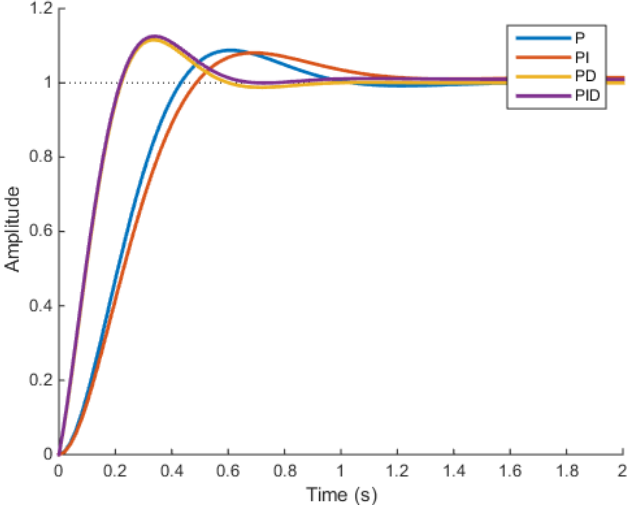
\includegraphics[width = 0.6\textwidth]{../img/diagram132.png}}
  \caption{}
\end{figure}
Selecting these parameters is known as \textbf{tuning}, and it was (and still is in machine learning circles) a very active area of research. These controllers are used everywhere, and can even be applied with acceptable results with little or no knowledge of the system being controlled!

If we set one of the gains to zero, then we remove that term from the controller, e.g. 
\begin{align}
  K_I \rightarrow 0 \textrm{ PID becomes PD controller}
\end{align}
Qualitatively, the three terms can be thought of as follows:
\begin{itemize}
  \item Proportional - tries to reach target as soon as possible
  \item Derivative - resists overshooting
  \item Integral - Corrects for steady state errors
\end{itemize}
Consider our servo model, each controller changes the step response in the following ways: 
\begin{figure}[H]
  \centerline{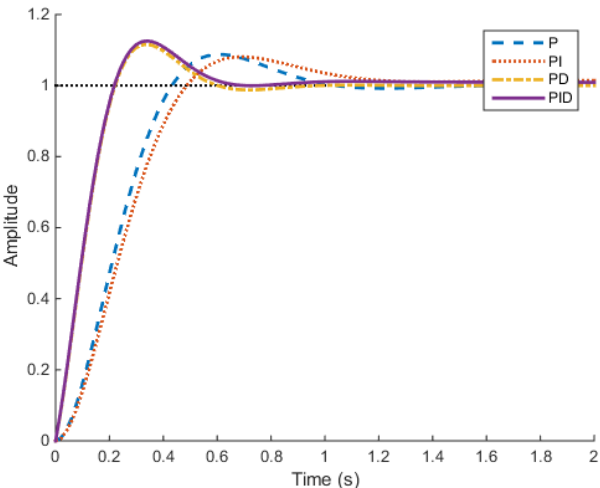
\includegraphics[width = 0.6\textwidth]{../img/diagram133.png}}
  \caption{}
\end{figure}
P - Initially chosen to give $\zeta$ close to 0.7 for acceptable transient response. PI - I term has little effect on the transient response for this \textbf{TYPE 1} system. Steady state error technically 0, but may improve in practice. Open loop transfer function:
\begin{equation}
  G(s)H(s) = \frac{\left(s-z_1\right) \left(s-z_2\right) \left(s-z_3\right)...}{s^p \left(s-\sigma_1\right) \left(s-\sigma_2\right) \left(s-\alpha_k + j \omega_k\right) \left(s- \alpha_k - j \omega_k\right)...}
\end{equation}
\begin{table}[H]
  \begin{center}
  \begin{tabular}{|c|c|c|c|}
    \hline
    & \multicolumn{3}{c|}{Input type}\\
    \cline{2-4}
    No. Integrators & Step & Ramp & Acceleration\\
    in denominator & $r(t) = a$ & $r(t) = at$ & $r(t) = \frac{at^2}{2}$\\
    = system TYPE & $R(s) = \frac{a}{s}$ & $R(s) = \frac{a}{s^2}$ & $R(s) = \frac{a}{s^3}$\\
    \hline
    \hline
    0 & $e_{ss} = \frac{a}{1+k_p}$ & $e_{ss} = \infty$ & $e_{ss} = \infty$\\
    \hline
    1 & $e_{ss} = 0$ & $e_{ss} = \frac{a}{k_v}$ & $e_{ss} = \infty$\\
    \hline
    2 & $e_{ss} = 0$ & $e_{ss} = 0$ & $e_{ss} = \frac{a}{k_a}$\\
    \hline
  \end{tabular}
  \end{center}
  \caption{}
\end{table}
PD - D term improves transient response as enabling higher P weighting to be used, but with a reduced overshoot. Steady state unchanged. PID - Again, transient response largely unchanged, but potential benefits in steady state. 
\subsection{Choosing the weightings}
The above figure was generated using a transfer function of a model of a servo system, and MATLAB's implementation of some commonly used "tuner" algorithms, where err on the side of caution.
\begin{quote}
  THESE ARE ONLY AS GOOD AS YOUR MODEL
\end{quote}
\subsection{PID control}
Implementing a basic PID controller is a comparatively simple task compared to that of analysing the system and choosing the coefficients. An example Arduino code is showing, assuming \textbf{Setpoint} determined elsewhere and \textbf{Input} receives the data from the feedback path.
\begin{verbatim}
  void Compute()
{
  /*How long since we last calculated*/
  unsigned long now = millis();
  double timeChange = (now - lastTime);

  /*Compute all the working error variables*/
  double error = Setpoint - Input;

  errSum = errSum+ (error * timeChange);

  double dErr = (error - lastErr) / timeChange;

  /*Compute PID Output*/
  Output = kp * error + ki * errSum + kd * dErr;

  /*Remember some variables for next time*/
  lastErr = error;
  lastTime = now;
}
\end{verbatim}
The process above is to get $\dif T$, calculate the error $E(s)$, update $\dif E \ \left(\frac{E(s)}{s}\right)$, est $\frac{\dif E}{\dif t} \ sE(s)$. We also know:
\begin{equation}
  G_c (s) = K_P + K_D s + \frac{K_I}{s}
\end{equation}
The new control signal \textbf{Output} is then sent to the system. This code could be used for a vast majority of simple applications, with the \textbf{input} and \textbf{output} and \textbf{set point}, being application specific. However, selecting the correct setpoint is easier said than done! In fact much of the field of robots could be seen (very cleverly) deciding \textit{what} the next set point should be. 
\end{document}